\documentclass[a4paper]{article}
\usepackage[utf8]{inputenc}
\usepackage[spanish, es-tabla, es-noshorthands]{babel}
\usepackage[table,xcdraw]{xcolor}
\usepackage[a4paper, footnotesep = 1cm, width=18cm, left=2cm, top=2.5cm, height=25cm, textwidth=18cm, textheight=25cm]{geometry}
%\geometry{showframe}

\usepackage{amsmath}
\usepackage{amsfonts}
\usepackage{amssymb}
\usepackage{float}
\usepackage{graphicx}
\usepackage{caption}
\usepackage{subcaption}
\usepackage{multicol}
\usepackage{multirow}
\setlength{\doublerulesep}{\arrayrulewidth}

\graphicspath{{../Ejercicio-1/}{../Ejercicio-2/}{../Ejercicio-3y4/}{../Ejercicio-5-6y7/}{../Ejercicio-8/}}

\usepackage{hyperref}
\hypersetup{
    colorlinks=true,
    linkcolor=blue,
    filecolor=magenta,      
    urlcolor=blue,
    citecolor=blue,    
}
\newcommand\underrel[2]{\mathrel{\mathop{#2}\limits_{#1}}}
\newcommand{\quotes}[1]{``#1''}
\usepackage{array}
\newcolumntype{C}[1]{>{\centering\let\newline\\\arraybackslash\hspace{0pt}}m{#1}}
\usepackage[american,oldvoltagedirection,siunitx]{circuitikz}
\usepackage{fancyhdr}
\usepackage{units}
\usepackage{booktabs}

\usepackage{tikz}
\usetikzlibrary{babel}

\pagestyle{fancy}
\fancyhf{}
\lhead{22.42 Laboratorio de Electrónica}
\rhead{Bertachini, Lambertucci, Londero Bonaparte, Mechoulam, Scapolla}
\rfoot{\center \thepage}

\begin{document}
\section{Puente de Wien - Medición de frecuencias}

\subsection{Introducción}

En esta sección, se procede a diseñar un puente de Wien, analizando las sensibilidades para todo el rango de medición.

Dicho puente permite conocer la frecuencia de una fuente desconocida, esto se debe a un procedimiento por el cual se comparan distintas magnitudes presentes en las ramas del puente, el cual se puede considerar como un proceso de medición indirecta. Existen limitaciones de tipo constructivas para el rango de frecuencias que se pueden medir, el asignado por la cátedra es de $10 \ kHz$ a $200 \ kHz$.

Un puente se considera en equilibrio cuando el cociente entre la tensión en la salida del puente $V_D$ y la tensión del generador $V_G$ es nulo. Esto implica que, el cociente entre una impedancia y su opuesta, debe ser equivalente al otro par dentro del circuito. Esta hipótesis nunca se puede confirmar ya que es una afirmación de carácter netamente teórico, mientras que en la práctica nunca se obtiene una tensión nula debido tanto a la incerteza en los métodos de medición utilizados, mostrado en el Ejercicio 1, así como también a las sensibilidades propias de los componentes.

El puente de Wien cuenta con cuatro ramas. El primer par de ramas adyacentes cuentan con componentes puramente resistivos, el otro está formado por circuitos RC, uno en paralelo y otro en serie, como se puede apreciar en la Figura (\ref{fig:Puente_de_wien}).
\begin{figure}[H]
\centering
\includegraphics[scale=0.8]{Circuitos/Puente_de_Wien.pdf}
\caption{Puente de Wien planteado}
\label{fig:Puente_de_wien}
\end{figure}
%~Puente_de_wien

Las relaciones obtenidas para el mismo en condición de equilibrio son las siguientes:
\begin{equation}
\frac{R_1}{R_3}+\frac{C_3}{C_1}=\frac{R_2}{R_4}
\end{equation}
\begin{equation}
w=\frac{1}{\sqrt{C_1C_3R_1R_3}}
\end{equation}

Generalmente el diseño del puente se realiza considerando las frecuencias desconocidas de las fuentes a medir. Se fijan valores equivalentes para los capacitores, lo mismo sucede con sus resistencias asociadas, quedando de la forma $R_1=R_3=R$ y $C_1=C_3=C$.

De esta forma, queda definido $R_2=2R_4$. Además, reduciendo el cálculo de la frecuencia, se obtiene:
\begin{equation}
f=\frac{1}{2\pi RC}
\label{frec}
\end{equation}

Las resistencias relacionadas con los capacitores son las que se varia para definir el comportamiento del puente, las mismas tienen una sensibilidad asociada. Con dicha finalidad, se utilizan resistencias variables (presets). 

Partiendo de la fórmula para la sensibilidad dada por $\Delta V_D=V_G \ F \ \delta_{Z_i}=V_G \ F \ \frac{\Delta Z_i}{Z_i}$ siendo $i$ la i-ésima rama, se obtienen las siguientes sensibilidades para las resistencias variables $R_3$ y $R_1$:
\begin{equation}
\Delta V_{D_{R_1}}=V_g\left|\frac{SC_1R_1}{SC_1R_1+1}\right|\frac{\Delta R_1}{R_1}
\end{equation}
\begin{equation}
\Delta V_{D_{R_3}}=V_g\left|SC_3R_3+1\right|\frac{\Delta R_3}{R_3}
\end{equation}

Siendo $F$ el factor cabeza de puente, dado por:
\begin{equation}
\begin{split}
F=& \ \frac{A}{1+2A\cos(\theta_A)+A^2} \\
A=& \ \frac{Z_4}{Z_2}
\end{split}
\label{cabeza_de_puente}
\end{equation} 

\subsection{Desarrollo}

Como primera decisión de diseño se implementan dos presets por cada resistencia variable requerida, esto se debe a que uno sirve para ajuste grueso y el otro para uno fino, logrando de esta manera obtener una calibración más precisa, que permita reducir la sensibilidad. Además, se consideran las limitaciones propias de los valores comerciales.

Se decide utilizar un capacitor multicapa de $1 \ nF$. Para dicho componente, considerando las frecuencias planteadas anteriormente y utilizando (\ref{frec}), se necesitan valores de resistencias de $15,9 \ k\Omega$ y $795 \ \Omega$ respectivamente. Para el primer caso, se utilizan dos presets de $X \ \Omega$ y $X \ \Omega$, mientras que para el segundo, de $X \ \Omega$ y $X \ \Omega$.
\begin{center}
	\huge{\textcolor{red}{\textbf{PONER VALORES DE PRESETS.}}}
\end{center}

Se decide tomar los siguientes para las ramas puramente resistivas del puente, $R_4= 1 \ k\Omega$ y $R_2= 2 \ k\Omega$. Volviendo a (\ref{cabeza_de_puente}), se obtiene un valor cabeza de puente $A=\frac{1}{2}$, que da un $F=0.22$.

%Sensibilidades
\begin{figure}[H]
\centering
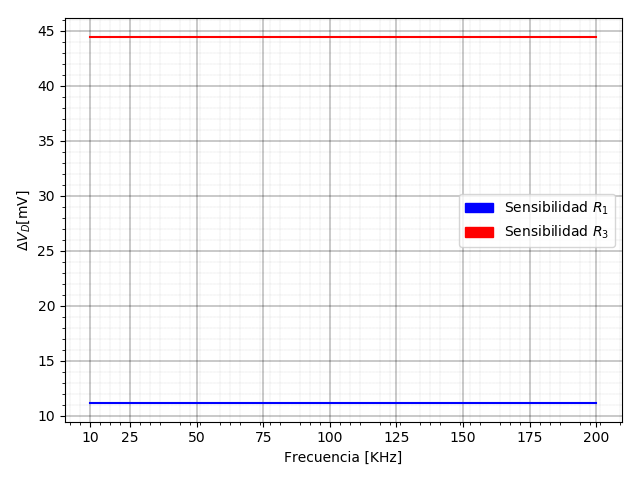
\includegraphics[scale=0.7]{Graficos/Sensibilidad}
\caption{Sensibilidades $R_1$ y $R_3$}
\label{fig:Sensibilidades}
\end{figure}
%~Sensibilidades



%Tension 10KHz
\begin{figure}[H]
\centering
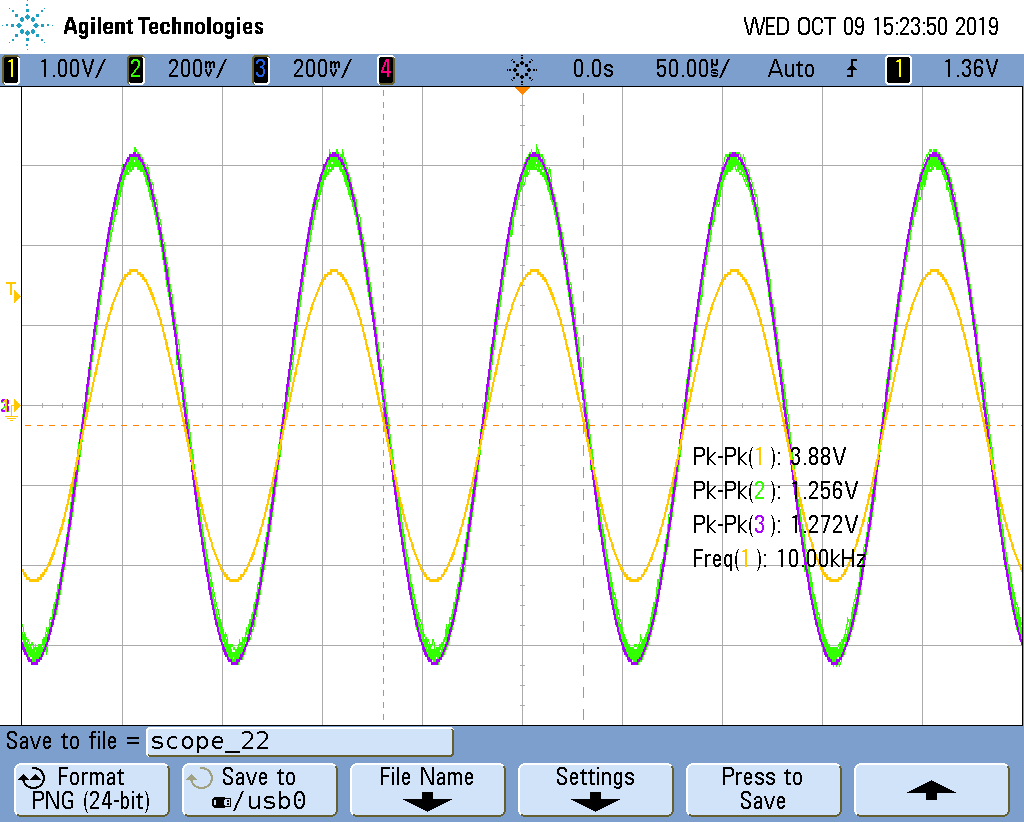
\includegraphics[width=0.8\textwidth,trim={0 3.45cm 0.1cm 1.75cm},clip]{Mediciones/Tensiones_10_KHz}
\caption{Tensión en $V_D$ a 10 kHz}
\label{fig:Tensiones_10_KHz}
\end{figure}
%~Tension 10KHz

%Tension 200KHz
\begin{figure}[H]
\centering
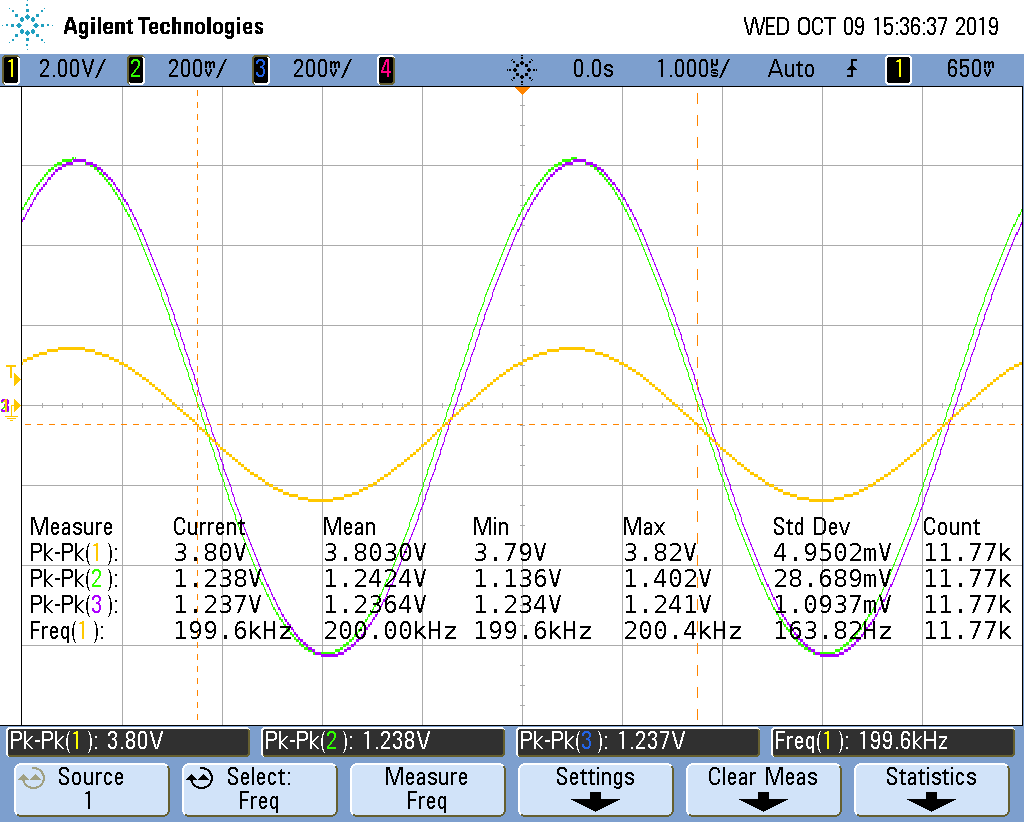
\includegraphics[width=0.8\textwidth,trim={0 3.45cm 0.1cm 1.75cm},clip]{Mediciones/Tensiones_200_KHz}
\caption{Tensión en $V_D$ a 200 kHz}
\label{fig:Tensiones_200_KHz}
\end{figure}
%~Tension 200KHz

\begin{table}[H]
\centering
\begin{tabular}{ccccc}
\hline
$\mathbf{f_g \ [kHz]}$ & $\mathbf{P_{R1} + P_{R2} \ [k\Omega]}$ & $\mathbf{P_{R3} + P_{R4} \ [k\Omega]}$ & $\mathbf{f_c \ [kHz]}$ & \textbf{Error [\%]} \\
\hline
10                     & 15.16                                  & 15.92                                  & 10.24                  & 2.45                \\
21.14                  & 7.53                                   & 7.95                                   & 20.57                  & 2.70                \\
44.7                   & 3.56                                   & 3.75                                   & 43.56                  & 2.55                \\
65.01                  & 2.58                                   & 2.45                                   & 63.30                  & 2.63                \\
94.55                  & 1.68                                   & 1.74                                   & 93.09                  & 1.55                \\
137.27                 & 1.159                                  & 1.187                                  & 135.69                 & 1.15                \\
165.69                 & 0.961                                  & 0.985                                  & 163.58                 & 1.27                \\
200                    & 0.8                                    & 0.82                                   & 196.98                 & 1.51   				\\
\hline            
\end{tabular}
\caption{Error entre frecuencia del generador y calculada}
\label{tab:Tabla_error}
\end{table}

\subsection{Conclusiones}

En la práctica, las resistencias que se suponen de igual magnitud como una condición inicial ($R_3$ y $R_1$), dejando de serlo como se puede apreciar en la Tabla (\ref{tab:Tabla_error}).
\begin{center}
	\huge{\textcolor{red}{\textbf{?????????????????}}}
\end{center}
Esto se debe a la variación de magnitud de los presets para poder llegar lo más cercano posible a la condición de equilibrio ($V_D=0$) considerando las sensibilidades previamente calculadas.
\begin{center}
	\huge{\textcolor{red}{\textbf{?????????????????}}}
\end{center}
Por otro lado, se observa que el error obtenido para el cálculo de la frecuencia es bajo, con un promedio de 1.97\%. Consecuentemente, se buscó otros valores de resistencias, bajo la misma frecuencia, con los que se pudiese llegar a la condición de equilibrio, descubriendo que existen dichos valores, pero obteniéndose un error más alto, encontrándose este entre el 25\% y 50\%. Dicha diferencia en el error, se debe a que, para llegar a esos resultados, se debe emplear impedancias más grandes.

\end{document}